\paragraph{Model merging is everywhere, but nobody knows the limit.}
Low-Rank Adaptation~\citep{hu2022lora} has made it routine to maintain
dozens of task-specific fine-tunes per base model; \emph{merging} them
into a single deployable model is now the dominant practical question,
with Task Arithmetic~\citep{ilharco2023task},
TIES~\citep{yadav2023ties}, DARE~\citep{yu2024dare},
KnOTS~\citep{stoica2025knots}, Task-Vector
Quantization~\citep{kim2025tvq}, and many successors competing on it.
Two operational questions go unanswered: \emph{how much room is left}
(a benchmark score says nothing about whether a better merger could
still halve its error) and \emph{when a method will fail} (a merger
that wins on one base can end up the worst on another with no
warning). Both reduce to a question no method
addresses: at a given storage budget, what is the best \emph{possible}
merging algorithm, and how far from it are today's methods?

\paragraph{Contribution in one sentence.} \emph{From a worst-task
rate-distortion analysis of LoRA merging we obtain two tools: a
merging method (\textsc{rd-encoder ridge}) with the lowest worst-task
loss of the ten methods we benchmark at default hyperparameters on
every base we test, and a CPU-only audit of any set of trained
adapters, taking minutes and no GPU, that predicts when classical
methods such as TIES flip from best to worst; its predictions held on
all three bases we tested, one of them
pre-registered\footnote{Throughout, \emph{pre-registered} means the
prediction was committed to our timestamped, version-controlled
experiment log \emph{before} the corresponding compute was run; an
anonymized bundle reproducing the commit trail is included in the
supplementary material.}.}

\begin{figure}[t]
\centering
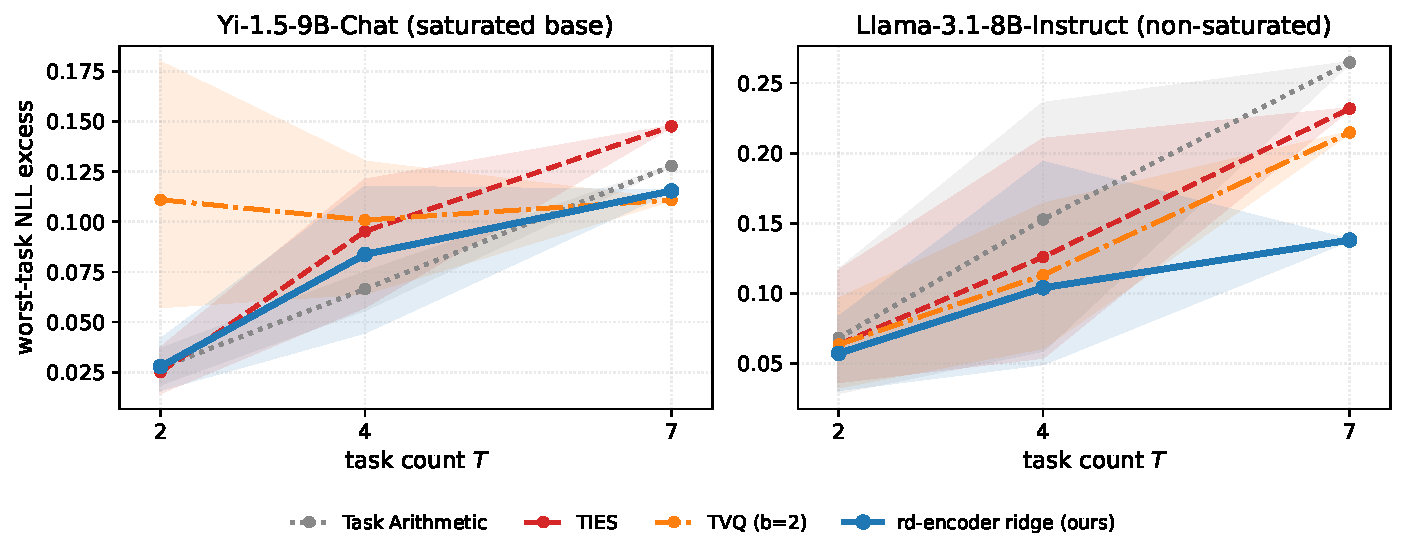
\includegraphics[width=0.78\textwidth]{figures/figure1_cross_model_T_scaling.pdf}
\caption{\textbf{Same merge methods, opposite outcomes across bases.}
Worst-task NLL excess vs.\ task count $T \in \{2, 4, 7\}$ on three
bases, ordered by $R$, the spread in per-task sign agreement that our
audit measures: saturated Yi-1.5-9B-Chat ($R = 0.077$), pre-registered
Mistral-7B-v0.3 ($R = 0.0326$), non-saturated Llama-3.1-8B-Instruct
($R = 0.028$); bands are per-subset min/max. Yi, above the predicted
window $[0.025, 0.075]$, inverts: TIES becomes \emph{worst} at $T = 7$
(\S\ref{subsec:exp-T-scaling}; threshold in
Appendix~\ref{app:sign-election-threshold}); Mistral, inside the
window, stays neither best nor worst, exactly as pre-registered.
\textsc{rd-encoder ridge} (ours) improves as tasks are added: its
excess falls from $0.84\times$ to $0.52\times$ Task Arithmetic's over
$T = 2 \to 7$ on Llama, and from $1.38\times$ to $0.47\times$ on
Mistral.}
\label{fig:hero}
\end{figure}

\paragraph{The lens: merging as compression.} Both tools come from
treating merging as lossy compression: $T$ task-specific weight
updates must be encoded into one model within a storage budget, and
quality is the extra held-out loss (negative log-likelihood, NLL) paid
by the \emph{worst}-affected task. For this problem we prove a
rate-distortion theorem: lower and upper bounds that match in their
rate exponent and split the worst-task error into an
\textbf{irreducible floor}, set entirely
by how much the task subspaces overlap and beyond the reach of any
encoder at any bit budget, plus a \textbf{compression term} that
decays exponentially in the bit budget and that an explicit encoder
achieves up to a constant. Measuring the overlap on $16$ trained LoRA
adapters (four bases $\times$ four tasks) settles which regime real
merging occupies: task subspaces are linearly \emph{independent} in
every layer of every model, so the floor is exactly zero and the
$0.10$--$0.22$ nats/token the five standard methods leave on the table
is recoverable algorithmic slack, not an information-theoretic cost. Zero overlap also predicts which methods
can work: subspace-alignment merging (KnOTS~\citep{stoica2025knots})
has nothing to exploit and is statistically indistinguishable from
naive averaging, while TIES, which attacks sign-level interference
instead, is the only baseline that separates. What \S\ref{sec:exp}
validates on real LLMs is thus the regime \emph{diagnosis}, not the
quantitative rate-distortion curve.

\paragraph{Contributions.}
\begin{enumerate}[leftmargin=*,topsep=2pt,itemsep=2pt]
\item \textbf{A merge method and an adapter audit, both falling out of
the bound (\S\ref{sec:exp}).} \textsc{rd-encoder ridge}, the encoder
from our achievability proof repaired by a single ridge term after a
measured spectral failure, has the lowest worst-task excess of all
ten methods at default hyperparameters on every base we test (a tuned
RegMean edges it on one saturated base;
\S\ref{subsec:exp-rd-encoder}). A
perturbation analysis of the TIES sign election yields a CPU-only audit
and a five-rule decision tree that predict when classical mergers flip
from best to worst, with the window's upper edge and its ambiguous
interior confirmed on three bases (one pre-registered).

\item \textbf{A rate-distortion theorem for worst-task merging
(\S\ref{sec:lower}--\S\ref{sec:achv}).} A reduction identity
(Lemma~\ref{lem:id}) splits worst-task distortion into a quantization
term around the $H$-weighted centroid plus a spread term no encoder
can remove; under the random-subspace hard distribution the spread
term equals $B^2(1 - \deff/(Tr))$ exactly
(Lemma~\ref{lem:floor-general}). At rate $R$, no encoder/decoder pair
beats this floor plus
$c_{\mathrm{TQ}} (B^2 \deff/(Tr))\, 2^{-2R/\deff}$, for arbitrary
positive-definite per-task spectra (Theorem~\ref{thm:general}). In
the floor-zero regime an explicit encoder (randomized orthogonal
mixing followed by scalar quantization) achieves the same
$2^{-2R/(Tr)}$ decay, so
$\mathcal{D}^\star = \Theta(B^2\, 2^{-2R/(Tr)})$ for fixed $T$
(Theorem~\ref{thm:achv}); the measured \emph{logarithmic} growth of
the constant in $T$ is posed as a sharp open problem
(Remark~\ref{rem:tgap}).

\item \textbf{A real-LLM calibration that turns the bound into a
measured gap (\S\ref{sec:exp}).} Floor zero everywhere;
$0.10$--$0.22$ nats/token of recoverable headroom; and a universal
``less-is-more'' dip at $2$-bit task-vector quantization on all four
architectures.
\end{enumerate}

\paragraph{Scope.} The bound certifies a \emph{lower envelope}, not a
tight per-instance grade: real task vectors are more benign than the
worst case, so a method's measured gap to $\mathcal{D}^\star$ is an
upper estimate of its true suboptimality. The matching upper bound is proved in the generic
random-subspace regime with $Tr \leq d$; the floor-positive regime has
an exponent gap we leave open (Remark~\ref{rem:sharedv-gap}).
\S\ref{sec:setup} formalizes the model; \S\ref{sec:lower} proves the
lower bound; \S\ref{sec:achv} gives the matching construction;
\S\ref{sec:exp} reports the empirical studies; \S\ref{sec:discussion}
discusses the cross-entropy bridge and limitations.
